%! TEX program = LuaTeX

\documentclass[nobackground,dvipsnames,table,aspectratio=169]{beamer}
\usepackage{cs152}

\mode<presentation>
{\usetheme{Hannover}
    \usecolortheme{cs152}
    \setbeamercovered{transparent}
    \useinnertheme[shadow=false]{rounded}
    \usebackgroundtemplate{}
    \setbeamercolor*{frametitle}{parent=palette primary}
    \setbeamerfont{block title}{size={}}
    \setbeamertemplate{navigation symbols}{}
}

\title{Designing for Trust and Safety}
\subtitle{CS 152 --- Trust and Safety Engineering}

\author[A. Stamos]{Alex Stamos}
\institute[Stanford University]{Stanford Cyber Policy Center}
\date[2022]{\today}
\subject{CS 152 --- Trust and Safety Engineering}
%\titlegraphic{
\includegraphics[width=5cm]{img/cyber-logo-white-black-red-WEB}}

% Change the level of bulleting on the ToC page
\setcounter{tocdepth}{2}

\graphicspath{{img/lesson02}}

%TODO OVERVIEW
%Formatting issues

\begin{document}

\begin{frame}
    \titlepage
\end{frame}

\section{Word of the Day: qwerty}

\begin{frame}{What Will You Learn Today?}
    \begin{itemize}
        \item The lifecycle of a trust and safety issue
        \item The basics of measuring badness
        \item The tradeoffs inherent in metrics
        \item How metrics can impact product design
    \end{itemize}
\end{frame}

\section{Measurement}

\begin{frame}{Need for Measuring Badness}
    \centering
    Without proper measurement, abuse fighting is shooting in the dark. \\~\\
    \begin{columns}[T]
        \small
        \column{0.3\textwidth}
            \centering
            Evaluate the size of badness.\\
            \begin{figure}
                
\includegraphics[width=0.75\textwidth]{size-of-badness}
            \end{figure}
        \column{0.3\textwidth}
            \centering
            Evaluate the efficiency of badness fighting.\\
            \begin{figure}
                
\includegraphics[width=0.75\textwidth]{efficiency-of-badness-fighting}
            \end{figure}
        \column{0.3\textwidth}
            \centering
            Evaluate the impact of badness.\\
            \begin{figure}
                
\includegraphics[width=0.75\textwidth]{impact-of-badness}
            \end{figure}
    \end{columns}
\end{frame}

\begin{frame}{Why Should We Evaluate the Size of Badness?}
    \begin{columns}[T]
        \column{0.45\textwidth}
            \centering
            \small{Develop the abuse fighting strategy based on biggest abuse vectors for a product/service.}
            \begin{figure}
                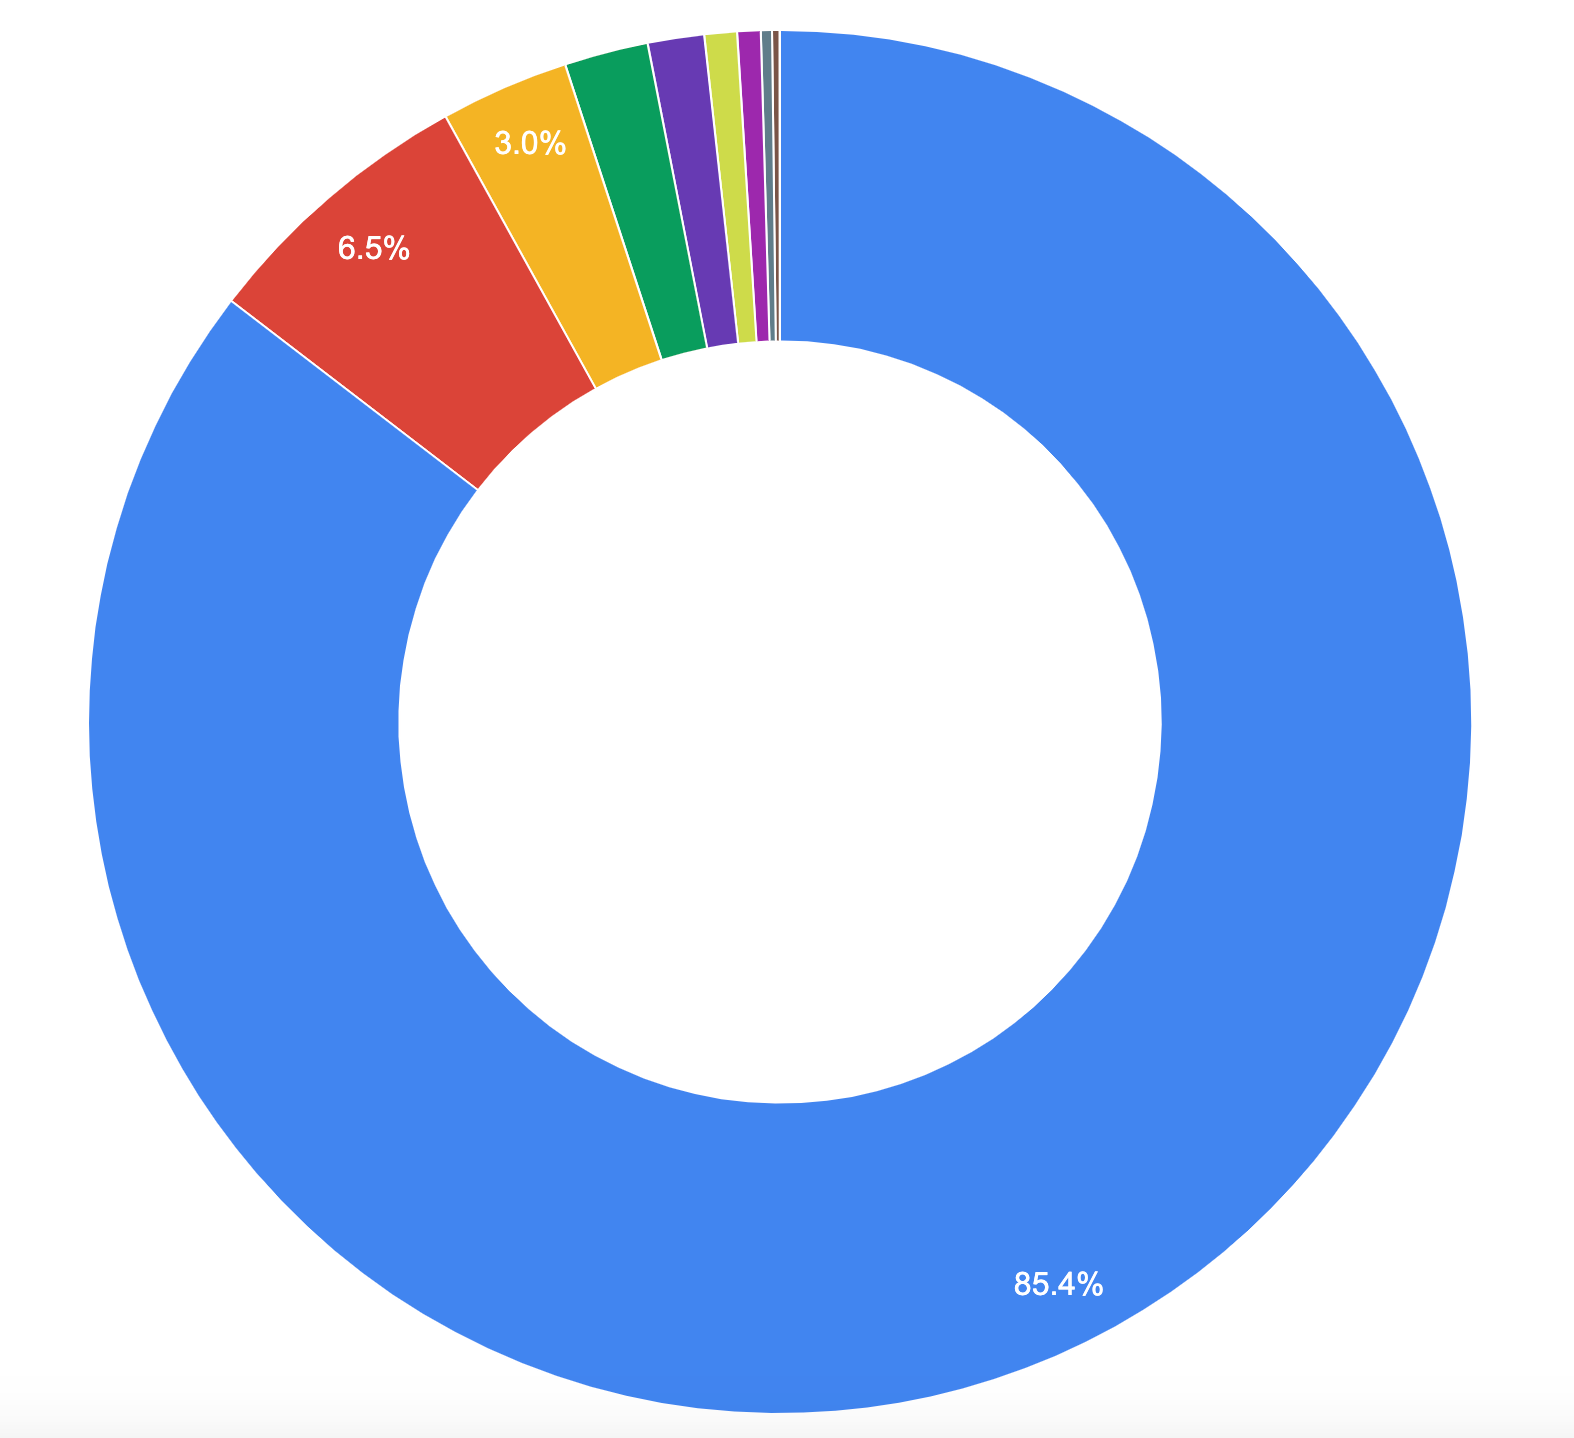
\includegraphics[width=\textwidth]{abuse-vectors}
                
\includegraphics[width=1.25\textwidth]{abuse-vectors-key}
            \end{figure}
        \column{0.55\textwidth}
            \centering
            \small{Reporting back to community on prevalence and actions taken.}
            \begin{figure}
                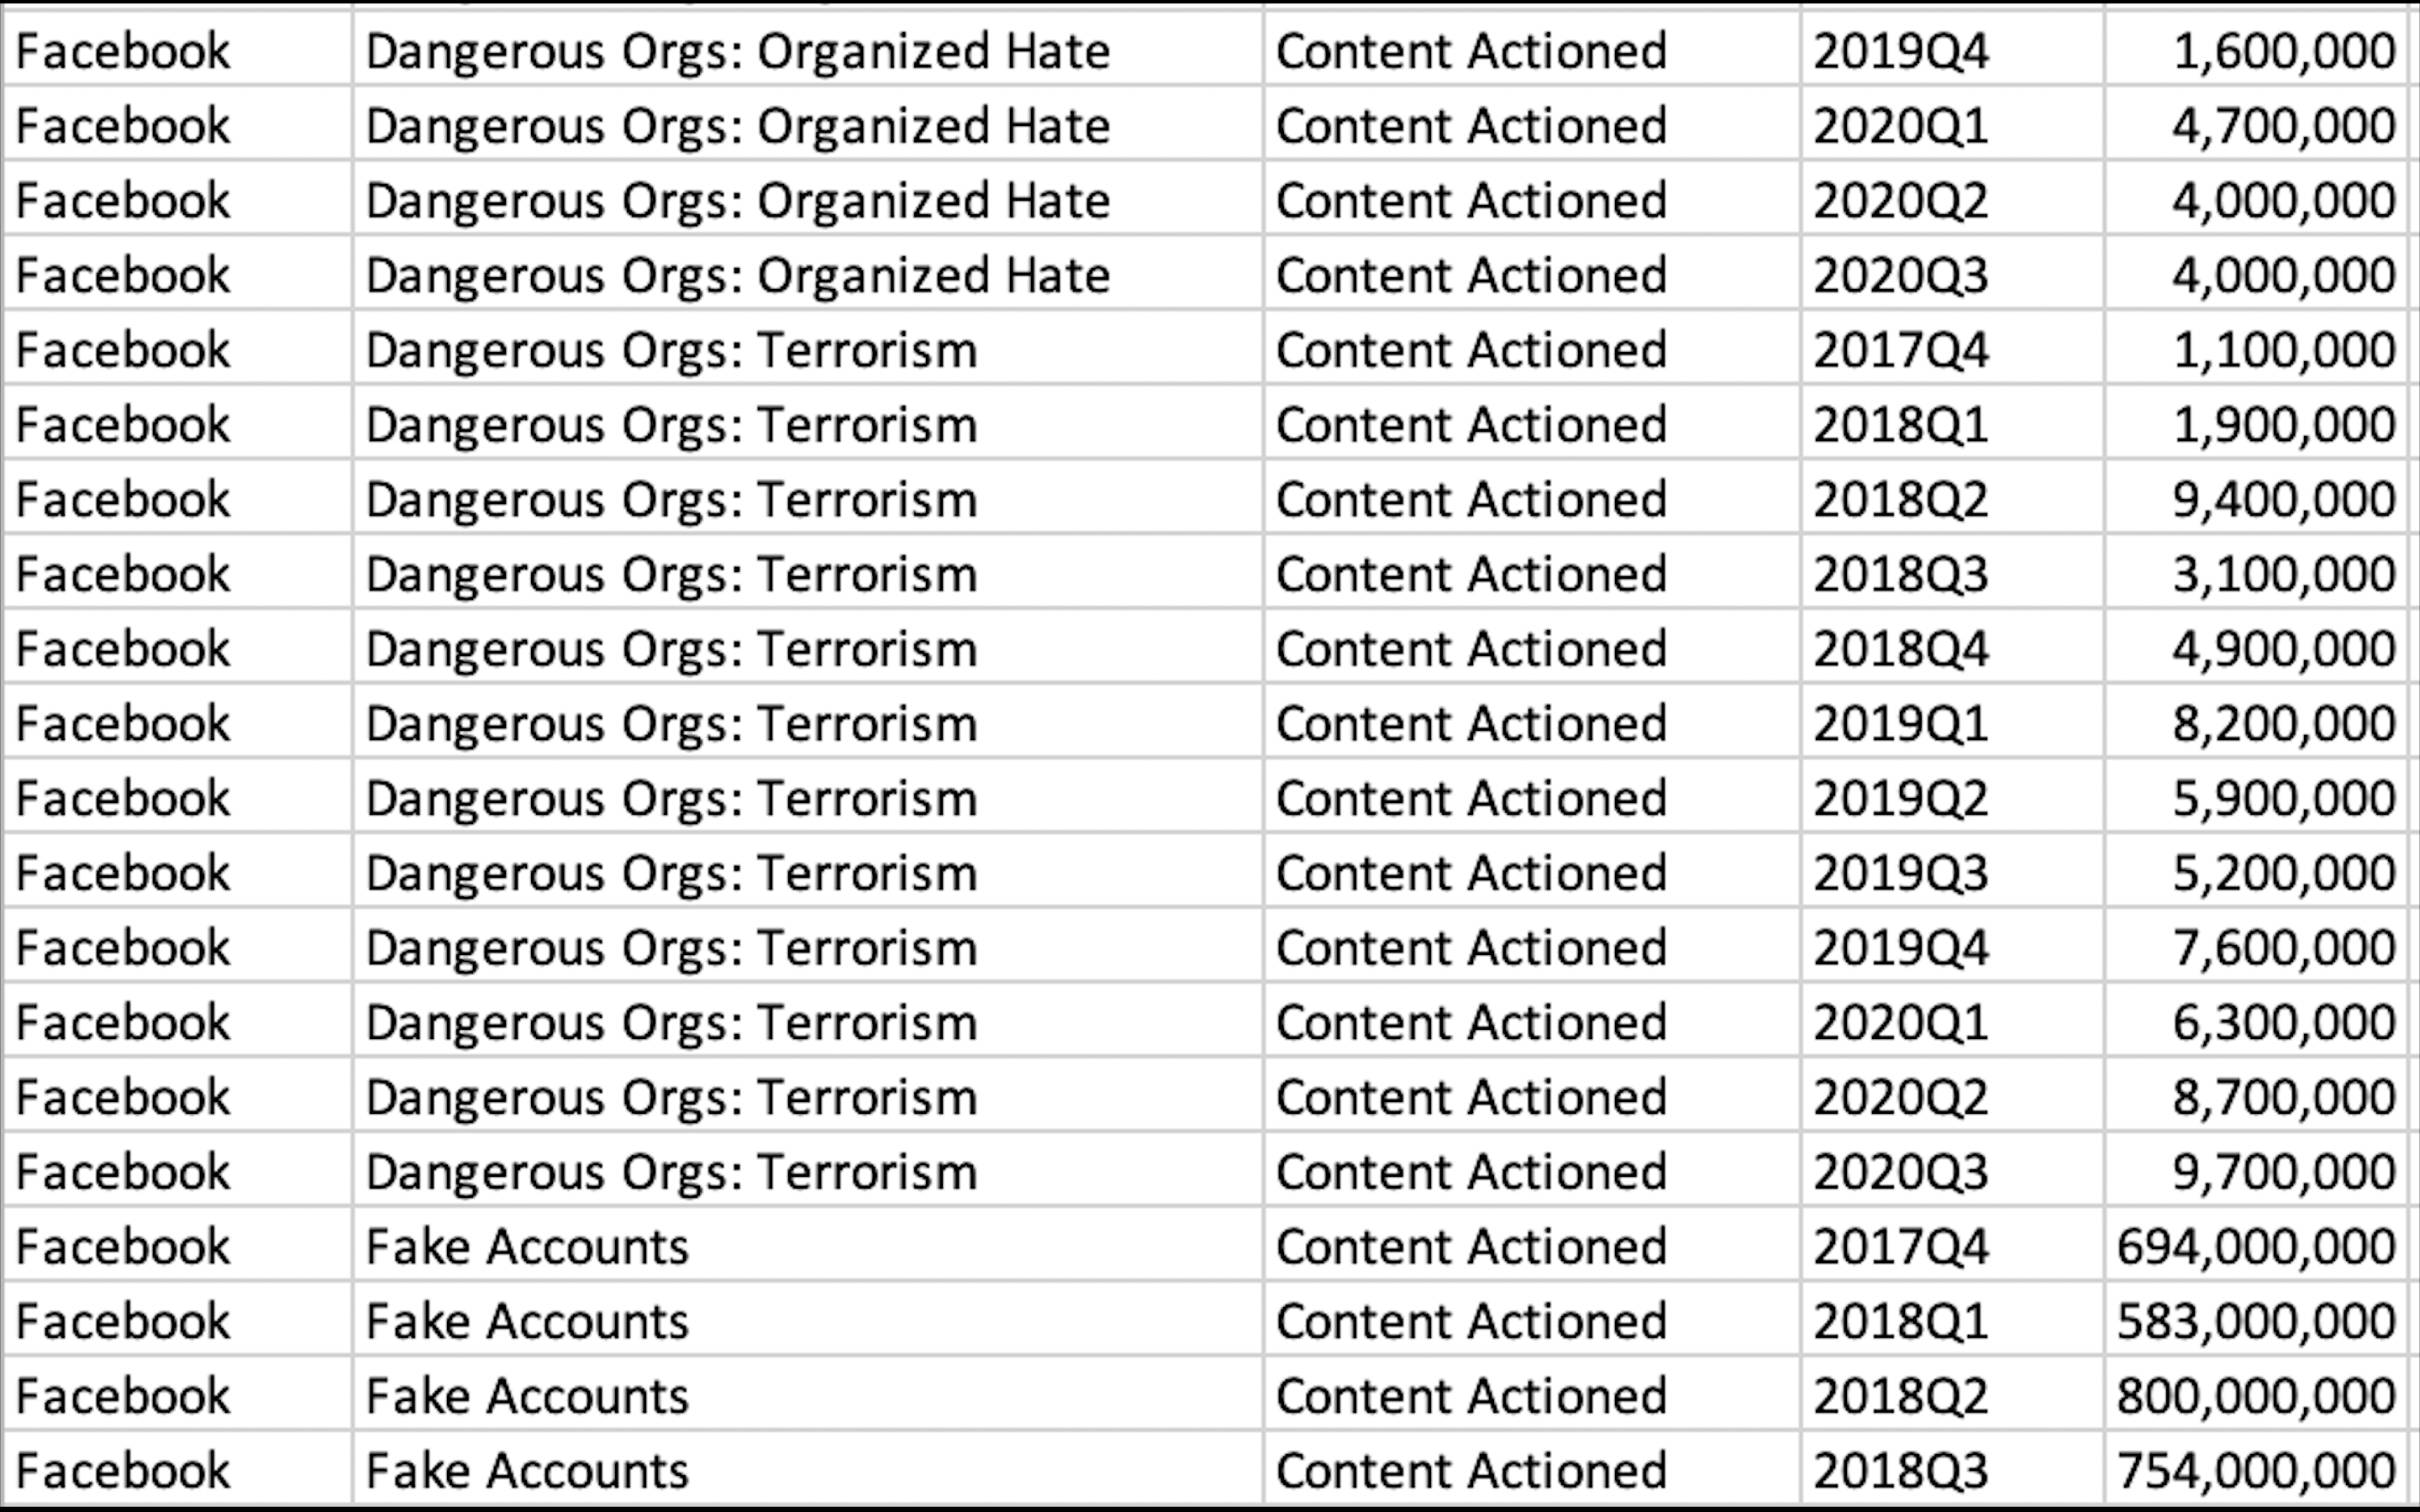
\includegraphics[width=\textwidth]{facebook-community-reports}
            \end{figure}
    \end{columns}
\end{frame}

\begin{frame}{Percentages may seem low, but absolute numbers may be high}
    \begin{figure}
        \centering
        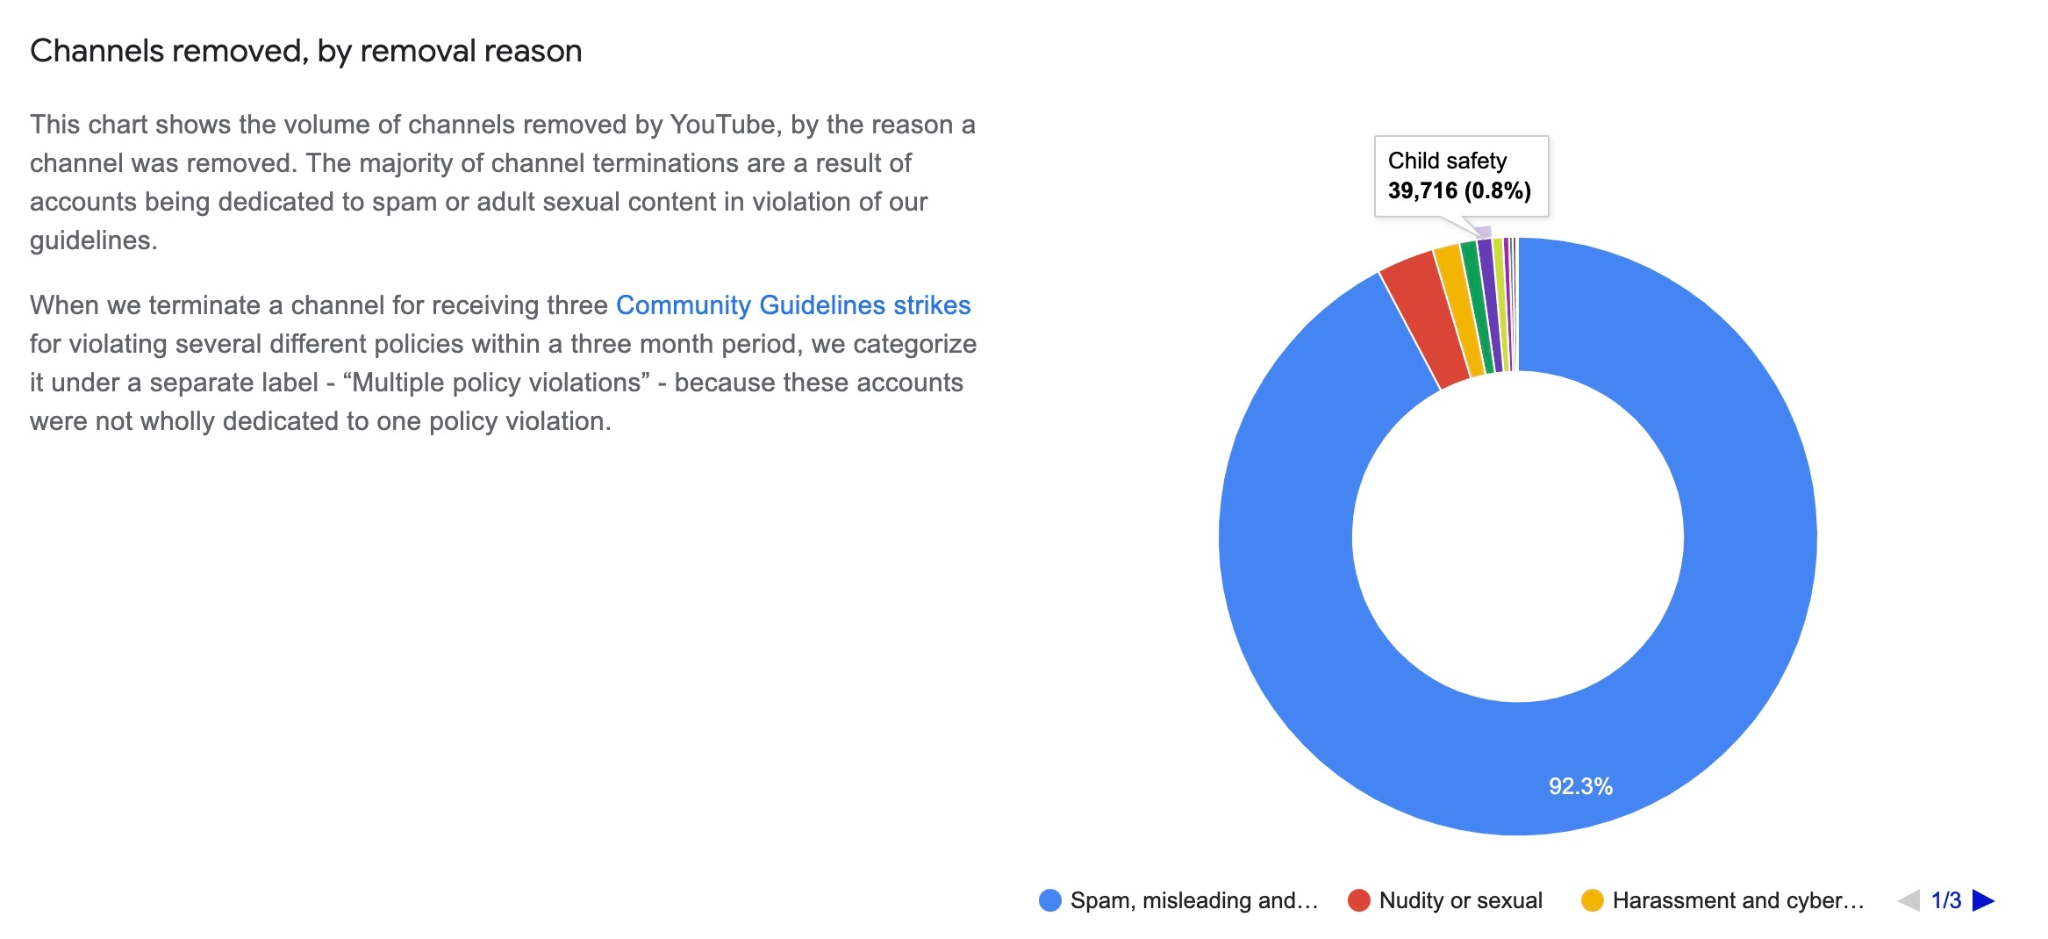
\includegraphics[width=\textwidth]{low-percentage-high-absolute}
    \end{figure}
\end{frame}

\begin{frame}{Why Should We Evaluate the Efficiency of Badness Fighting?}
    \begin{columns}[T]
        \column{0.6\textwidth}
            \centering{Refining and adapting abuse fighting strategy based on efficiency.}
            \begin{figure}
                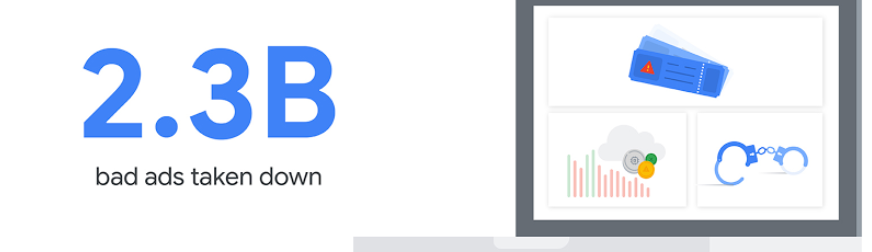
\includegraphics[width=\textwidth]{bad-ads-taken-down}
            \end{figure}
            \tiny
            2.3 billion bad ads in 2018 for violations of both new and existing policies, including nearly 207,000 ads for ticket resellers, over 531,000 ads for bail bonds and approximately 58.8 million phishing ads. \\~\\

            Google  introduced \textbf{31 new ads policies} in 2018 to address abuses in areas including third-party tech support, ticket resellers, cryptocurrency and local services such as garage door repairmen, bail bonds and addiction treatment facilities.
        \column{0.4\textwidth}
            \centering
            Building efficient and scalable ML models.\\
            \begin{figure}
                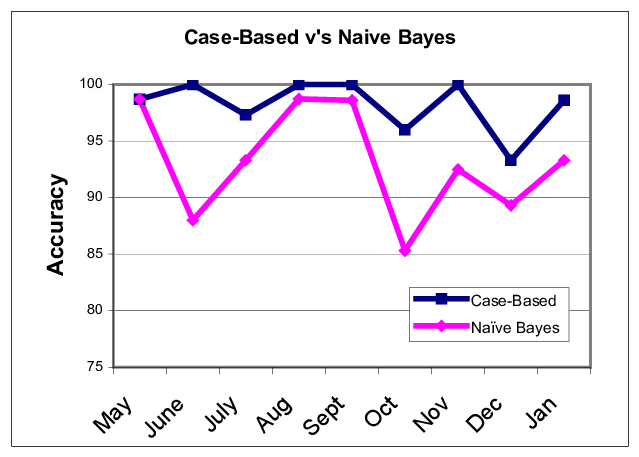
\includegraphics[width=\textwidth]{case-based-vs-naive-bayes}
            \end{figure}
    \end{columns}
\end{frame}

\begin{frame}{Why Should We Evaluate the Impact of Badness?}
    \centering
    Badness leads to poor user experience, has impact on user trust and in some cases leads to user harm.\\~\\
    \begin{columns}[T]
        \column{0.5\textwidth}
            \centering
            \small{Human flags by flagging reason (YouTube Transparency Report)}
            \begin{figure}
                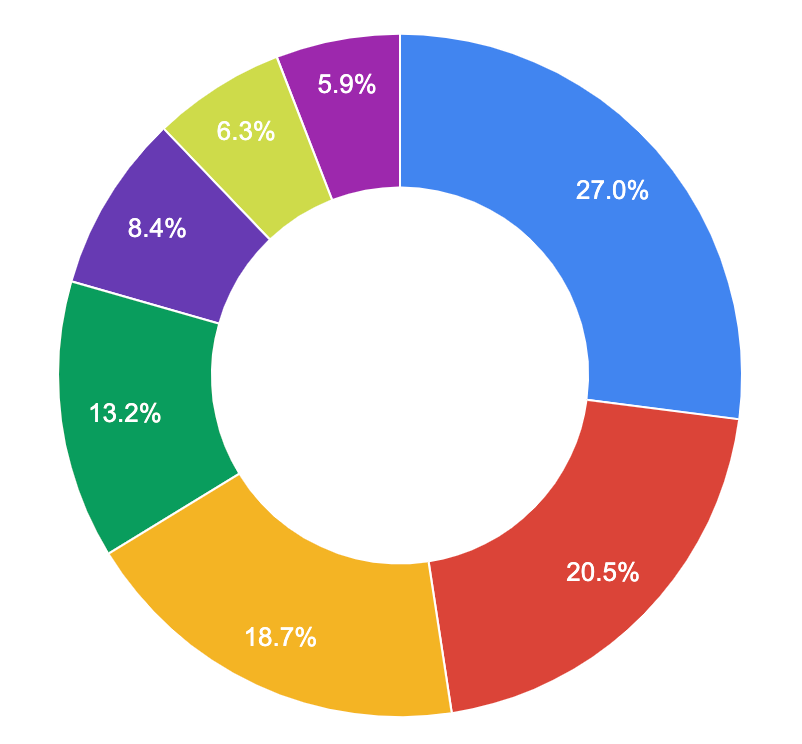
\includegraphics[width=\textwidth]{youtube-reports}
                
\includegraphics[width=1.5\textwidth]{youtube-reports-key}
            \end{figure}
        \column{0.5\textwidth}
            \centering
            \small{Top user harms that results from a data breach}
            \begin{figure}
                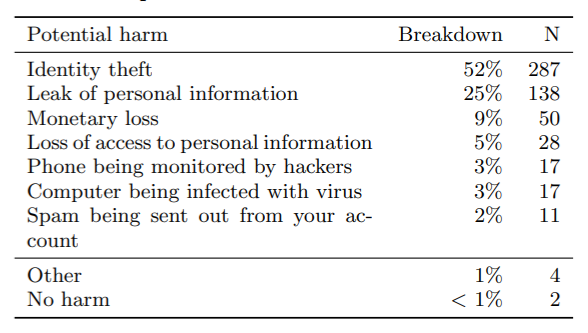
\includegraphics[width=\textwidth]{potential-harms}
            \end{figure}
    \end{columns}
\end{frame}

\begin{frame}{Measurement Methods}
    \begin{columns}[T]
        \column{0.5\textwidth}
            \Large{Internal Methods} \\
            \begin{itemize}
                \item Collecting and measuring \\
                \item Sampling \\
                \item Behavioral metrics \\
            \end{itemize}
        \column{0.5\textwidth}
            \Large{External Methods} \\
            \begin{itemize}
                \item Crawling and scraping \\
                \item Crowdsourcing \\
                \item User metrics \\
                \item User experience studies \\
            \end{itemize}
    \end{columns}
\end{frame}

\begin{frame}{} %TODO2 make video/image cover sidebar
    \thispagestyle{empty}
    \href{https://www.youtube.com/watch?v=REWeBzGuzCc}{
\includegraphics[width=\paperwidth]{unknown-unknowns}}
\end{frame}

\begin{frame}{False Positives and False Negatives}
    Let us take the example of a binary email spam classifier, in which each email can be either spam or not spam.
    
    \textbf{Confusion matrix}
    \begin{tabularx}{0.8\textwidth}{|c|c|c|}%TODO2 make table fit on page. currently only changing the lines of the table and not adjusting text
        \hline
        & \textbf{Predicted: Real Email} & \textbf{Predicted: Spam Email} \\
        \hline
        \textbf{Actual: Real Email} & True Negatives (TN) & False Positives (FP)\\
        \hline
        \textbf{Actual: Spam Email} & False Negatives (FN) & True Positives (TP) \\
        \hline
    \end{tabularx}
\end{frame}

\begin{frame}{Precision and Recall: a Tug of War} %TODO2 - make less cursed
    \footnotesize
    \textbf{Precision} = $$\frac{True Positive}{True Positive + False Positive}$$ the proportion of positive identifications that are correct\\
    \textbf{Recall} = $$\frac{True Positive}{True Positive + False Negative}$$ the proportion of actual positives that were identified correctly\\
    \textbf{Accuracy} = $$\frac{Number of Correct Predictions}{Total Predictions}$$ the fraction of predictions the model got right\\
    \textbf{Prevalence} = $$\frac{False Negative}{Total}$$ the proportion of bad content that got past your system
    \begin{figure}
        \centering
        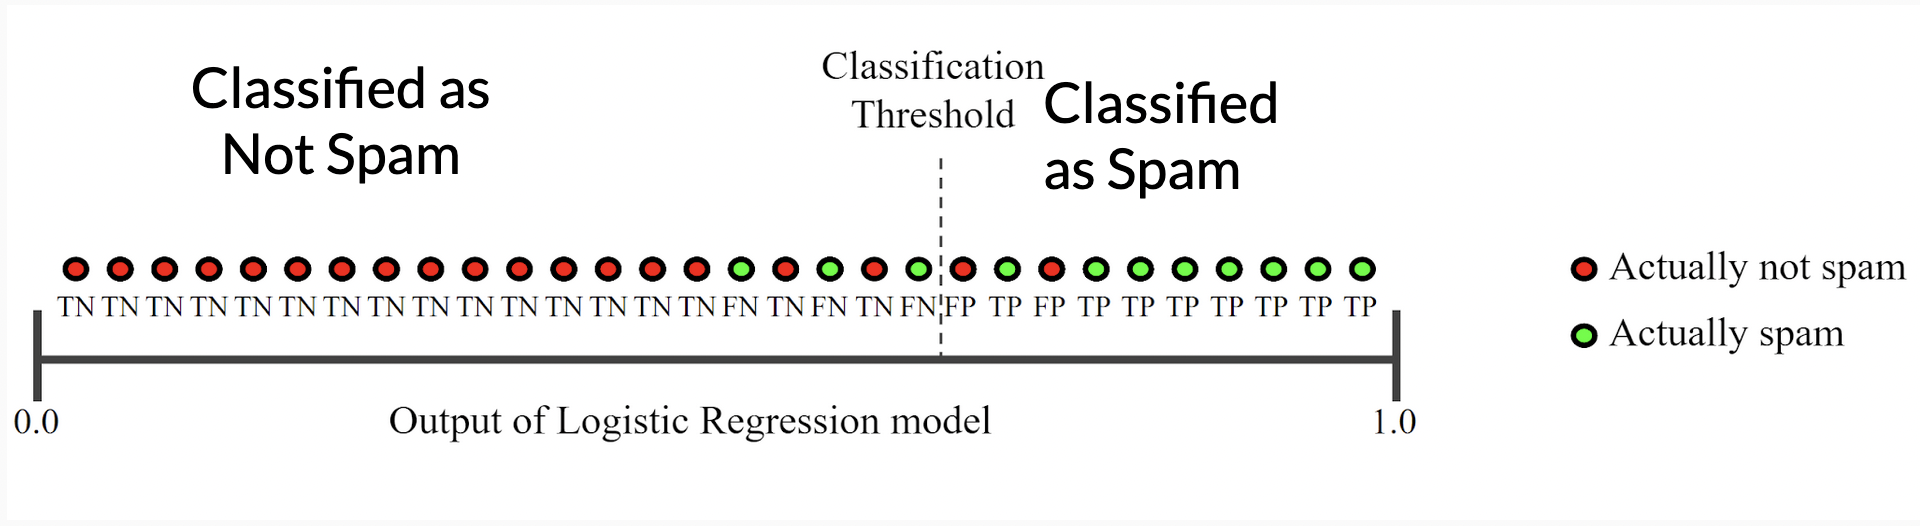
\includegraphics[width=0.75\textwidth]{spam-classification}
    \end{figure}
\end{frame}

\begin{frame}{Problem of Long-tails}
    \begin{columns}
        \column{0.6\textwidth}
            \begin{figure}
                \centering
                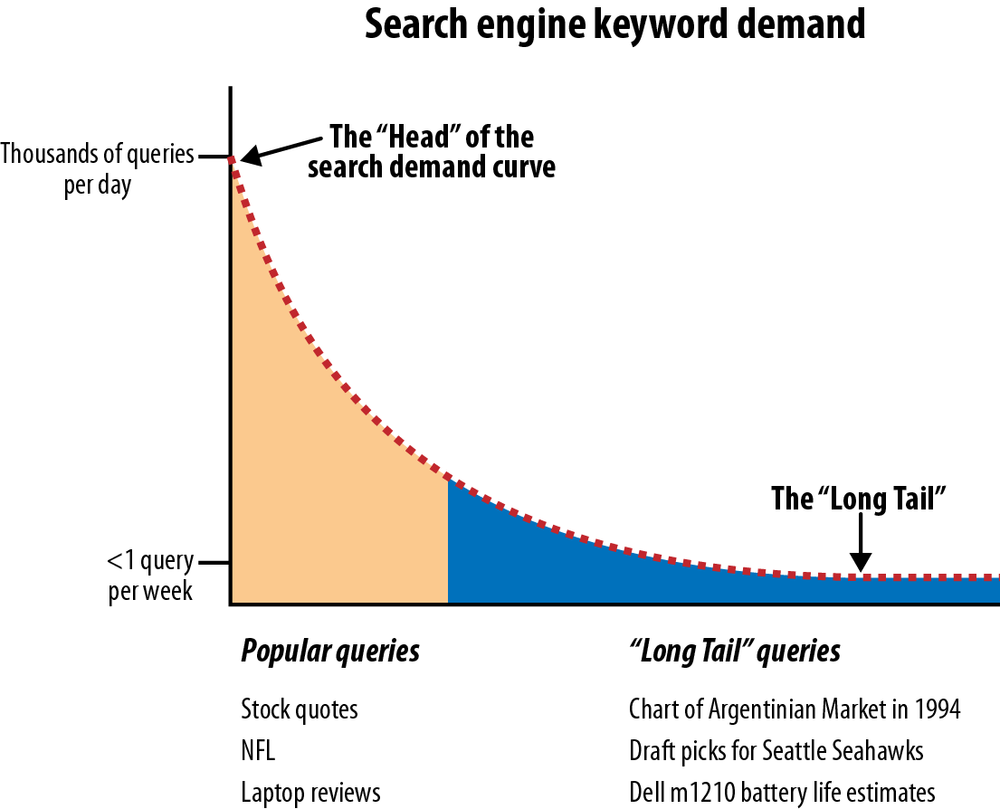
\includegraphics[width=\textwidth]{long-tail}
            \end{figure}
        \column{0.4\textwidth}
            The majority of online searches comprise unique rather than popular queries. \\~\\
            \begin{itemize}
                \item Videos that get less than 10 viewers \\~\\
                \item Blog post that have zero followers \\~\\
                \item Websites that show up on the 10th page of the search results
            \end{itemize}
    \end{columns}
\end{frame}

\begin{frame}{Prevalence}
    \textbf{Prevalence} = \% of bad content that got past your system 
\end{frame}

\begin{frame}{Measurement Summary}
    \centering
    \textit{“Two basic principles of management, and regulation, and life, are:} \\~\\
    
    \textit{You get what you measure.} \\~\\
    
    \textit{The thing that you measure will get gamed.”} \\~\\
          - Matt Levine, Bloomberg 
\end{frame}

\begin{frame}{Metric Perversity}
    Metrics are supposed to help you make good decisions
    \vspace{0.05\textheight}
    \begin{itemize}
        \item Are your metrics respectful?
        \item Are they perverse?
        \item Will they cope with rare, important failures?
        \item Are they robust to data collection issues?
    \end{itemize}
    \vspace{0.1\textheight}
    \centering
    \large
    \textbf{Many safety problems come from bad metrics}
\end{frame}

\begin{frame}{Using Measurements to Make Decisions}
    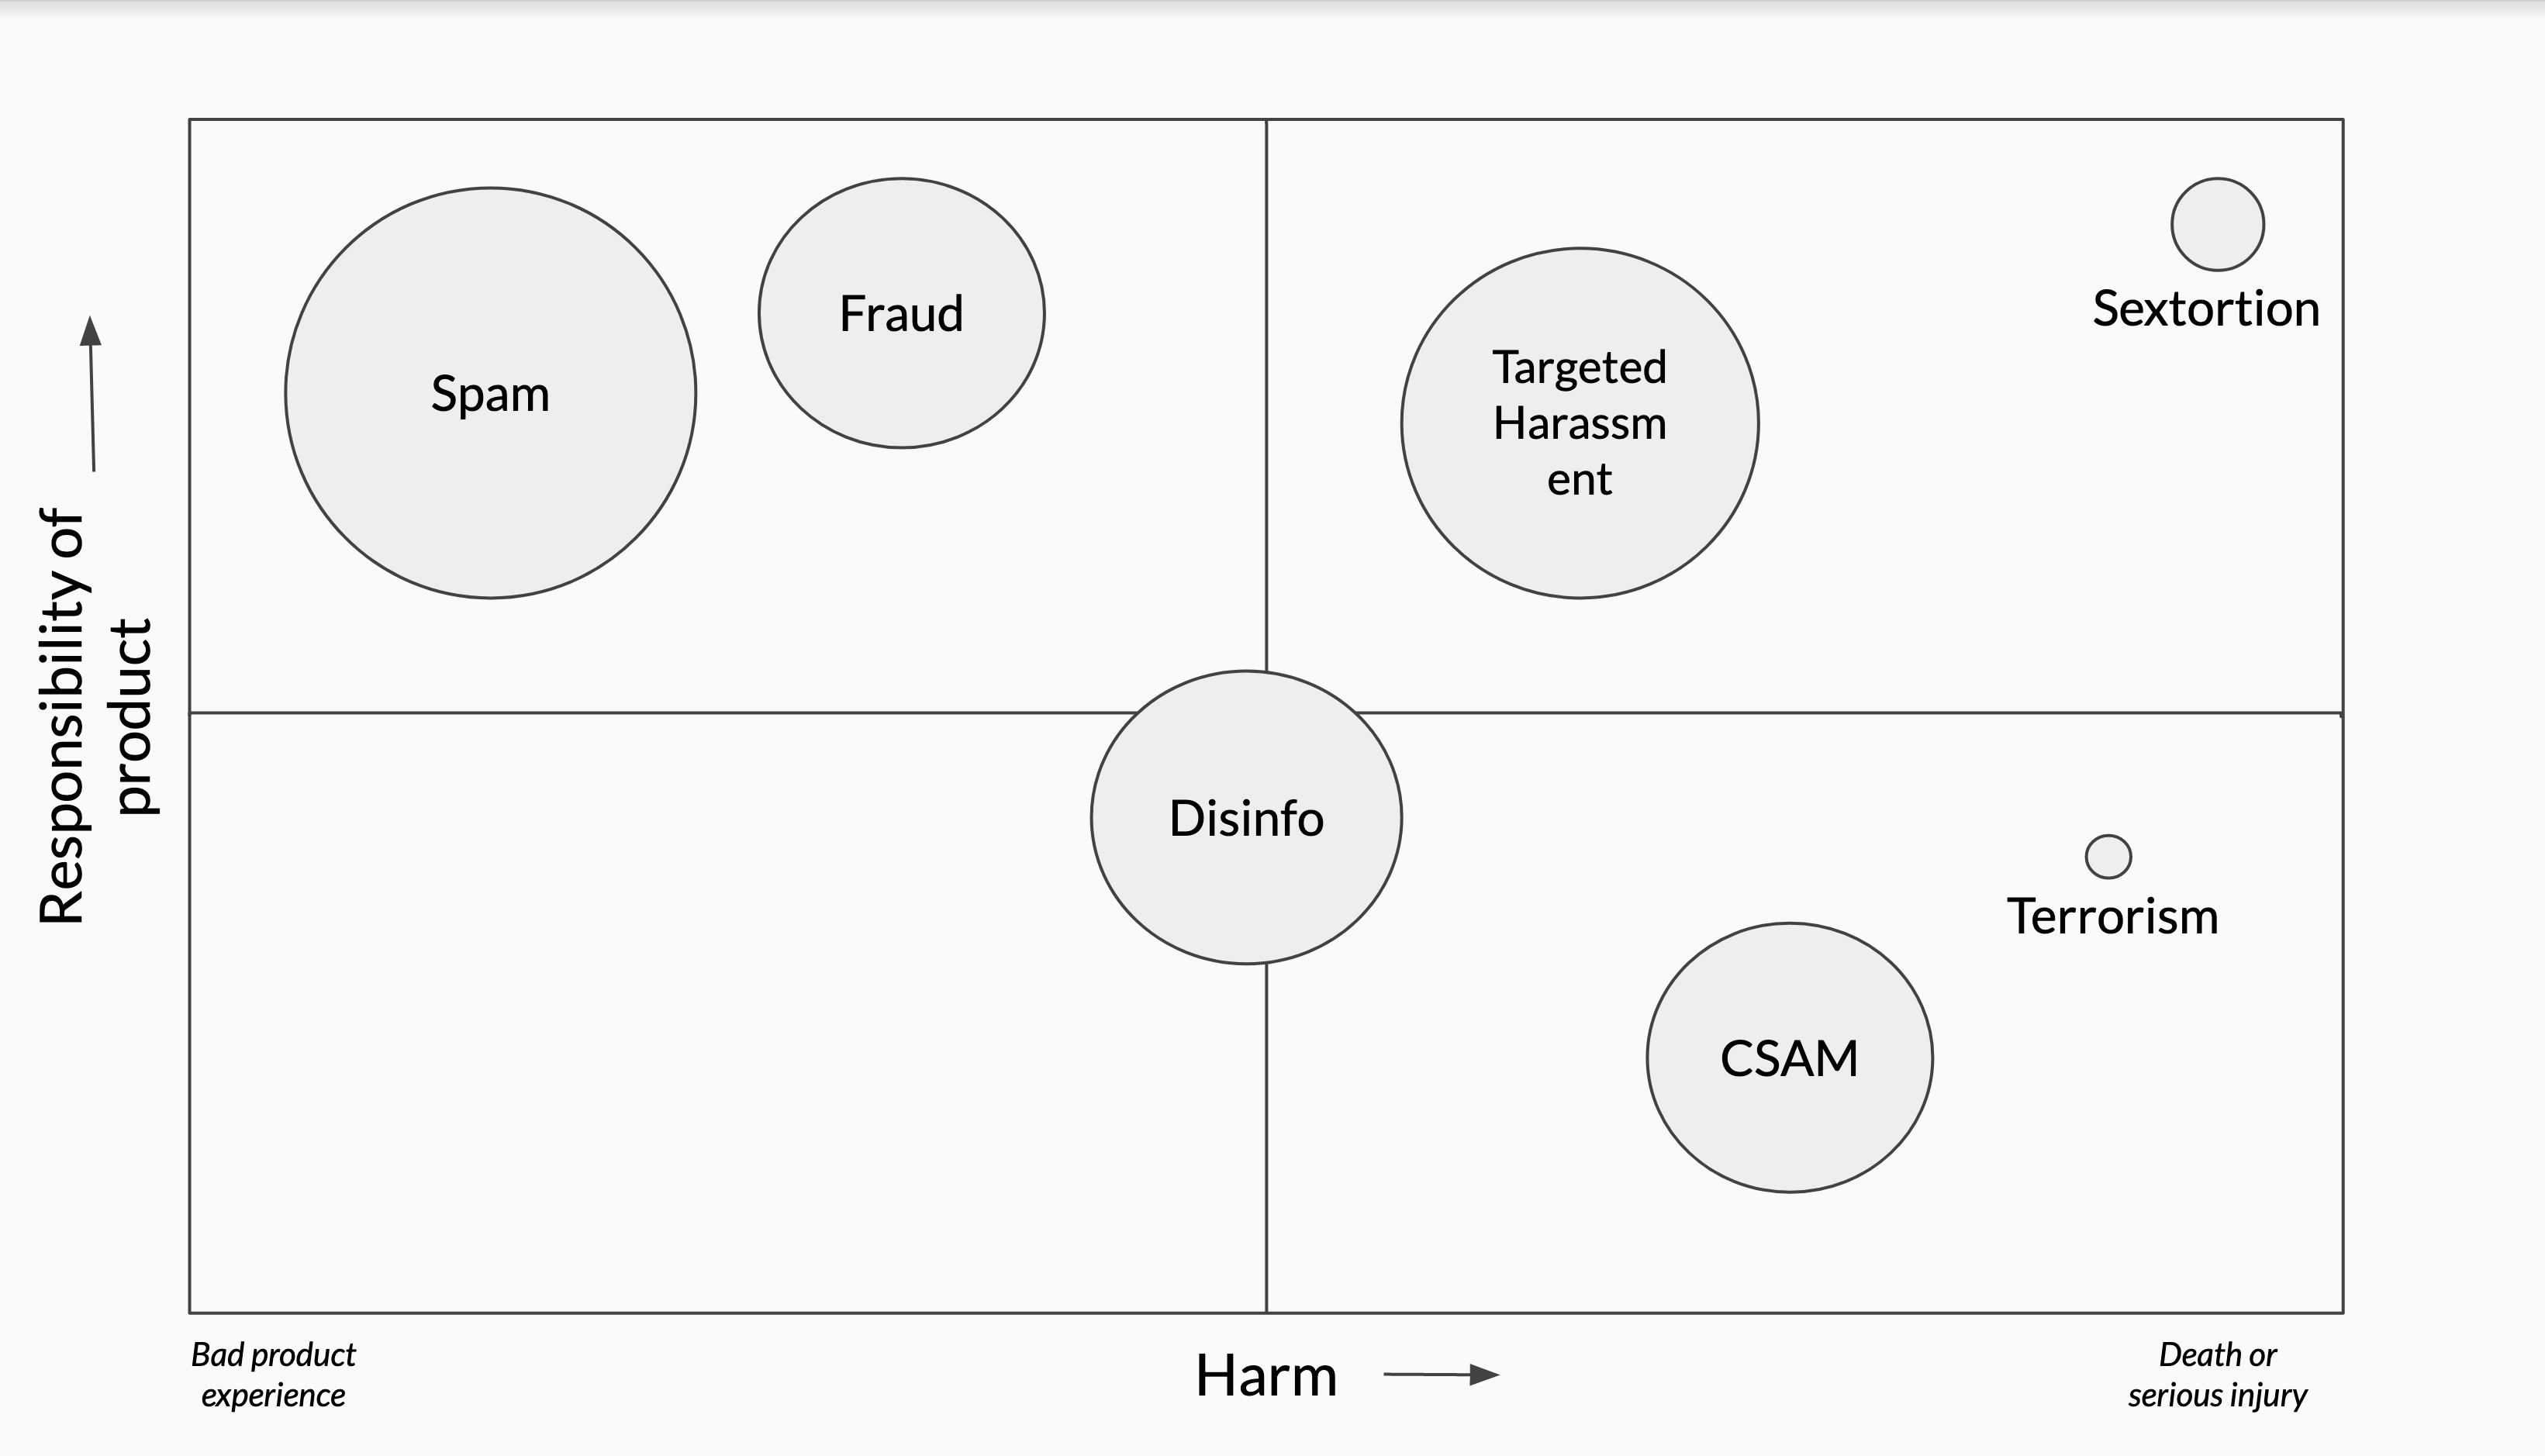
\includegraphics[width=\textwidth]{responsibility-vs-harm}
\end{frame}

\begin{frame}{Prioritization in Trust and Safety}
    \centering
    The \textbf{level} of harm associated with an area of abuse\\~\\
    +\\~\\
    The \textbf{prevalence} of the abuse\\~\\
    +\\~\\
    The product’s \textbf{responsibility} for enabling such abuse\\~\\
    =\\~\\
    \large{Prioritization}
\end{frame}

\section{Activity}

\begin{frame}{ACTIVITY - Sort Badness}
    \begin{columns}[T]
        \column{0.4\textwidth}
            \begin{enumerate}
                \item Hateful comments on a blog posts
                \item Violent images on a photo sharing platforms \item Suicide how to videos on a video sharing platforms
                \item Clickbait ads on websites
                \item False stories from low-quality news sources
                \item Offensive words on reviews of Apps on a mobile store.
            \end{enumerate}
        \column{0.6\textwidth}
            \vspace{0.025\textheight}
            \small{Based on your understanding of the abuse types listed on the left, place them on the matrix below}
            \vspace{0.12\textheight}
            \begin{figure}
                \centering
                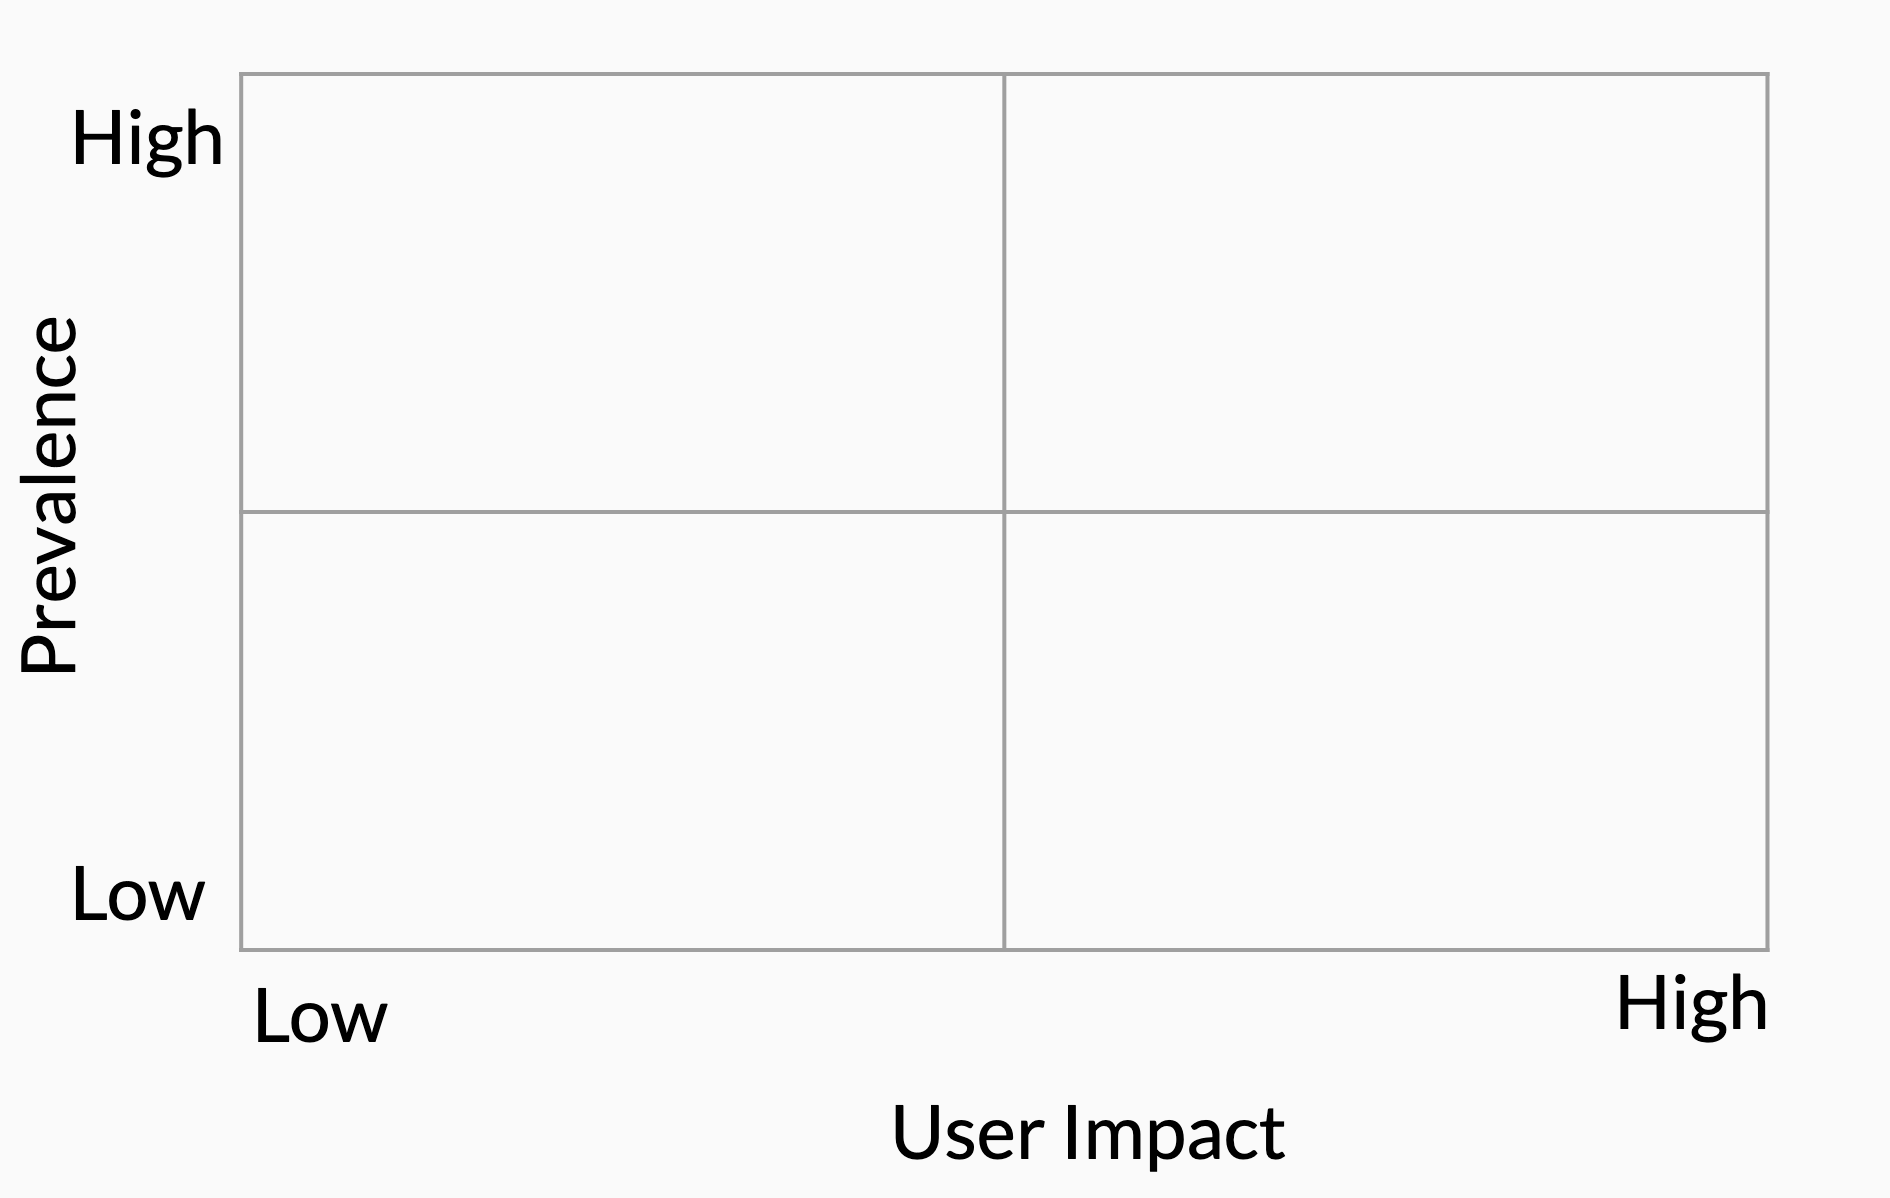
\includegraphics[width=\textwidth]{sort-badness}
            \end{figure}
    \end{columns}
\end{frame}

\section{Tradeoffs}

\begin{frame}{The Iron Triangle of Engineering}
    \centering
    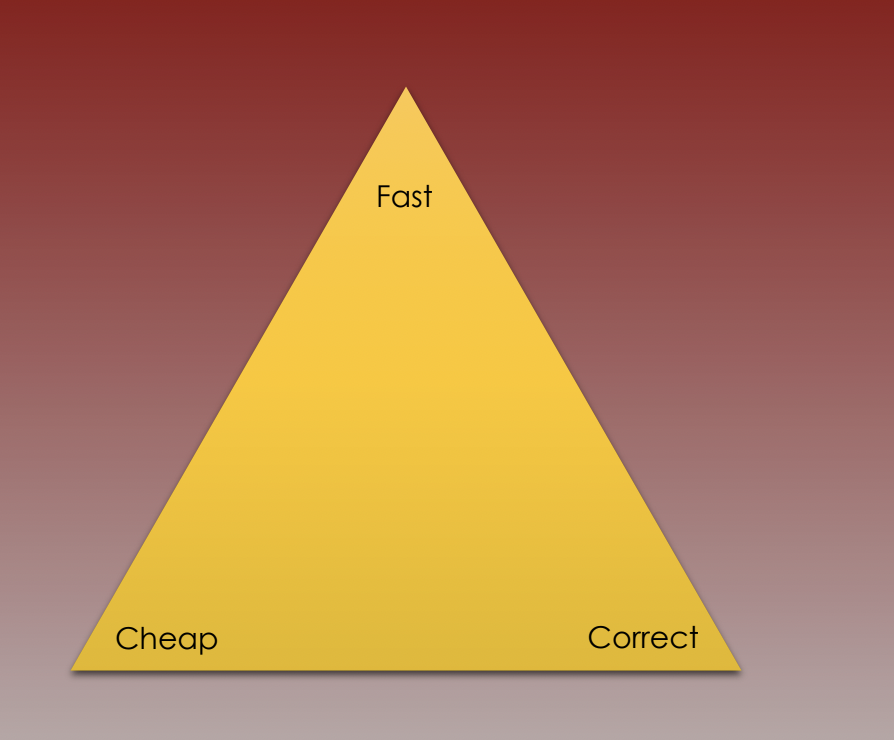
\includegraphics[height=0.9\textheight]{iron-triangle}
\end{frame}

\begin{frame}{The Stamos Tridecagram of Difficult Tradeoffs}
    \centering
    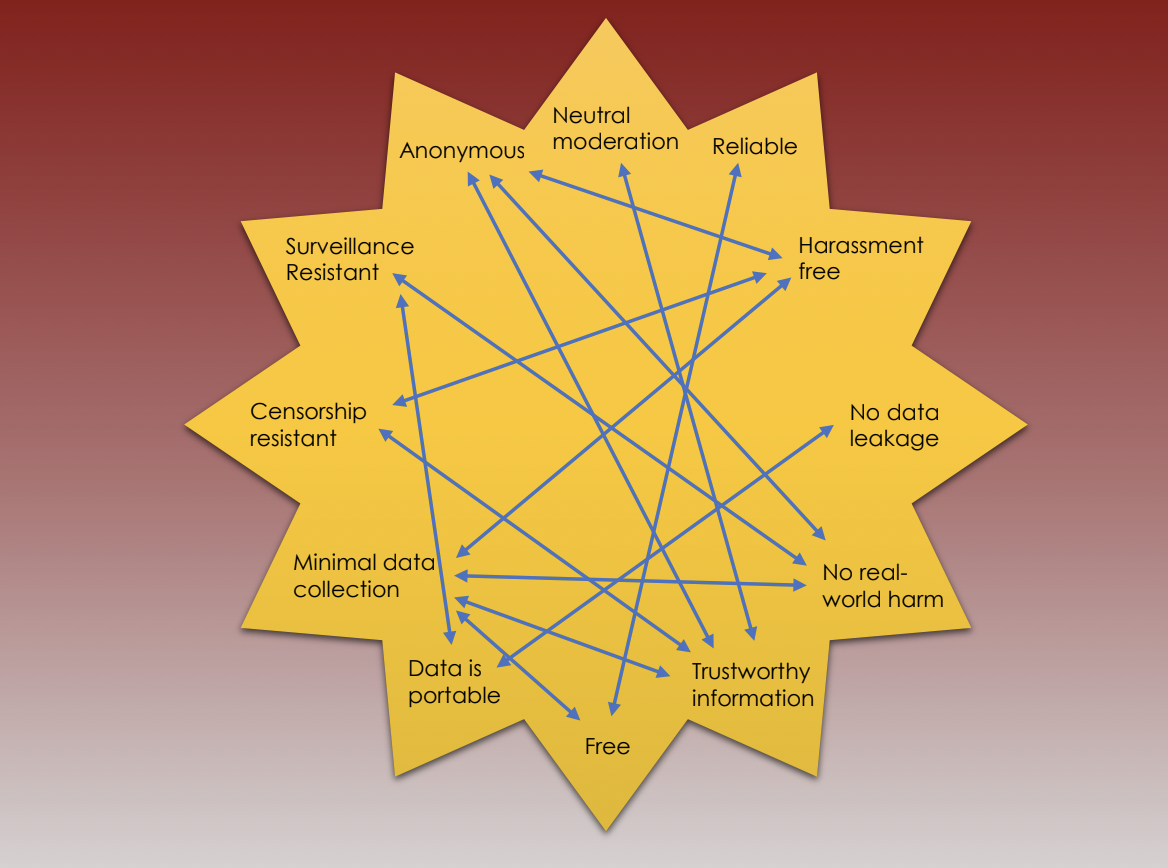
\includegraphics[width=\textwidth]{tridecagram.png}
\end{frame}

\begin{frame}{Inherent Tradeoffs}
    \begin{itemize}
        \item Under-Enforcement vs. Over-Enforcement
        \begin{itemize}
            \item E.g. privacy v. anti-abuse scanning 
            \item E.g. designating political terrorist groups
        \end{itemize}
        \item Legal Obligations vs. Awful but Lawful 
        \item Every company has finite resources
    \end{itemize}
\end{frame}

\end{document}
